% -*- TeX-master: "../fat_manual.tex" -*-

\section{Chalmers File Preparation}

  \subsection{GDS file}
   This next step is designed for all files. One needs to convert it to GDS
   
   \begin{enumerate}
   	\item \quote{Open} \textbf{\quote{Layout editor}} program;
   	\item \texttt{Load} the dxf file from above;
   	\item \texttt{Save as GDSII};
   	\item \texttt{Connect to MC2 sever (has the name 003 in it) \ira go to required folder and drop} so that it is in the system.
   \end{enumerate}

  \subsection{GDS to GPF}
   One needs to convert GDS to GPF in order for it to be read by the EBG500.
   \begin{enumerate}
   	\item \cmd{Log onto \quote{server005} from Terminal \ira type \quote{Beamer} and run \ira load a premade pattern};
   	\item There should be three blocks. \cmd{Double click on each block \ira check parameters \ira \quote{OK} \ira click \quote{run} button.}
   	\item Repeat for all three blocks.
   \end{enumerate}
  
  \subsection{Making cjob}
   Cjob is required by EBL systems, and this takes a bit more work. To begin with, one needs to have access to \texttt{GDS II} or GPF file created above.
   
   \begin{enumerate}
   	\item \texttt{Go to server} \ira \texttt{Type in "cjob"} to launch program and begin creating the EBL file.
   	\item \textbf{Create substrate} \texttt{Drag substrate box} \ira \texttt{Select type of substrate and set its size};
   	\item \textbf{Exposure parameters} \texttt{Drag exposure box to substrate box \ira Give name \ira Give \textbf{accelerating voltage} \ira Pre height measurement?} (whether to measure the height from eGUN or not) \ira \texttt{Tick \textbf{"Fixed global mark"} and enter coordinates of global marks, their type};
   	\item \textbf{Layout parameters} \texttt{Drag layout box \ira Choose the grid by selecting x and y units. Choose the step between the grids.} (The program will find the center of the wafer with the global marks. From (0,0) a symmetrical grid will be drawn out with defined parameters);
   	\item \textbf{Pattern parameters} \texttt{Drag pattern box\ira Load file that will be copied to each grid \ira Define the local marker positions.} (The program will store the location of these markers relative to the centre of each grid. When running, the marks will be found, center of each grid found from relative shift, and the pattern centered on the point found); \ira \texttt{Choose Dose to apply} (from data sheets) \ira \texttt{Choose current to deliver dose} \red{MUST BE GIVE A FREQUENCY <100MHZ};
   	\item \texttt{Export \ira choose "branch" to export \ira export job.} File can now be loaded into EBL.
   \end{enumerate}


 \subsection{How pattern is made}
  \begin{enumerate}
  	\item Define global markers and size of substrate;
  	\item From global markers, program draws a grid to create number of cells chosen. Wafer size determines grid size. Global markers determine grid position;
  	\item Center of each grid is treated at the origin (0,0). When defining local markers, they count off from this origin.
  \end{enumerate}

  Then, in the SEM the markers are used to
   \begin{enumerate}
   	\item Find global markers to determine grid location;
   	\item Move to each grid and find local marker \ira from the local marker, find the center of each grid.
   \end{enumerate}

  
  \begin{figure}[h]
	\centering
	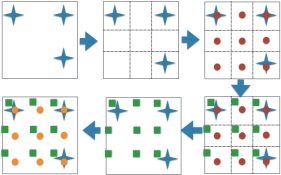
\includegraphics[width=0.55\linewidth]{pat}
	\label{fig:pat}
  \end{figure}

\newpage